\section{Dreiachsiger Spannungszustand\label{spannung:section:Dreiachsiger_Spannungszustand}}
\rhead{Proportionalität Spannung-Dehnung}
Wie im Kapitel Spannungsausbreitung beschrieben herrscht in jedem Punkt ein anderer Spannungszustand.
Um die Spannung im Boden genauer untersuchen zu können, führt man einen infinitesimales Bodenteilchen ein.
Das Bodenteilchen ist geometrisch gesehen ein Würfel.
An diesem Bodenteilchen trägt man die Spannungen ein in alle Richtungen.

\begin{figure}
	\centering
	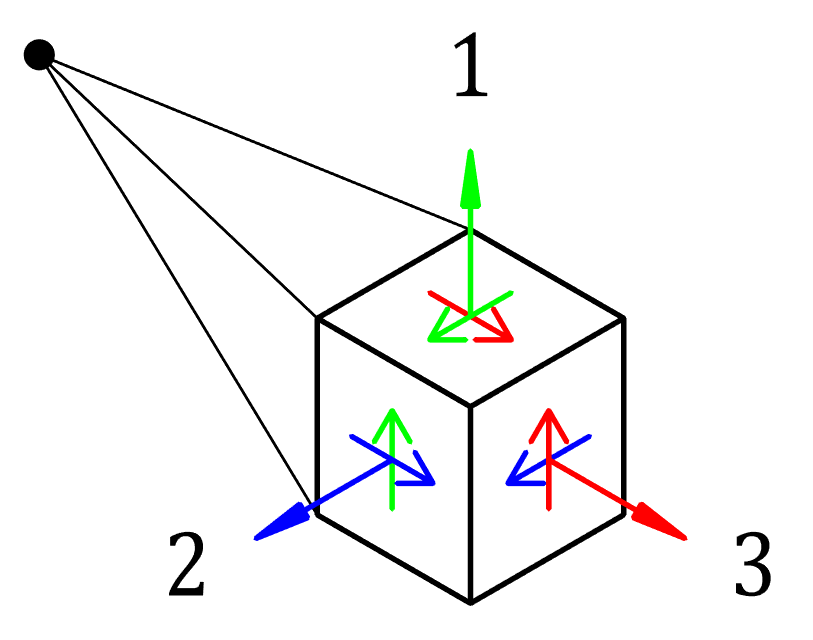
\includegraphics[width=0.5\linewidth,keepaspectratio]{papers/spannung/Grafiken/infinitesimalerWuerfel.png}
	\caption{Infinitesimales Bodenteilchen}
	\label{fig:infintesimaler-wurfel}
\end{figure}

An diesem infinitesimalen Bodenteilchen hat man ein räumliches Koordinatensystem, die Achsen $(1,2,3)$.
Die Achsen vom Koordinatensystem zeigen aus den 3 ersichtlichen Flächen heraus.
Pro ersichtliche Fläche haben wir eine Normalspannung und zwei Schubspannungen.
Im Gegensatz zum eindimensionalen Zustand entstehen bei einer Belastung des Bodenteilchens eine Vielzahl an Spannungen.
Es entstehen diverse Normal- und Schubspannungen.
Die Schubspannungen befinden sich an der Fläche, sie gehen rechtwinklig von den Achsen weg.
Die Schubspannungen auf einer Fläche stehen im 90 Grad Winkel zueinander.
Geschrieben werden diese mit $\sigma$, mit jeweils zwei Indizes.
Die Indizes geben uns an, in welche Richtung die Spannungen zeigen.
Der erste Index ist die Fläche auf welcher man sich befindet.
Der zweite Index gibt an, in welche Richtung die Spannung zeigt, dabei referenzieren die Indizes auch auf die Achsen $(1,2,3)$.
Bei den Spannungen sind immer positive als auch negative Spannungen möglich.
Es können also Druck- oder Zugspannungen sein.

Zunächst wird untenstehend der allgemeine Spannungszustand betrachtet.

Spannungstensor 2. Stufe i,j $\in$ {1,2,3}
\[
\overline{\sigma}
=
\sigma_{ij}
=
\begin{pmatrix}
	\sigma_{11} & \sigma_{12} & \sigma_{13} \\ 
	\sigma_{21} & \sigma_{22} & \sigma_{23} \\
	\sigma_{31} & \sigma_{32} & \sigma_{33}
\end{pmatrix}
=
\qquad
\Rightarrow
\qquad
\vec{\sigma}
=
\begin{pmatrix}
	\sigma_{11}\\
	\sigma_{12}\\
	\sigma_{13}\\
	\sigma_{21}\\
	\sigma_{22}\\
	\sigma_{23}\\
	\sigma_{31}\\
	\sigma_{32}\\
	\sigma_{33}
\end{pmatrix}
\]

Dehnungstensor 2. Stufe k,l $\in$ {1,2,3}

\[
\overline{\varepsilon}
=
\varepsilon_{kl}
=
\begin{pmatrix}
	\varepsilon_{11} & \varepsilon_{12} & \varepsilon_{13} \\ 
	\varepsilon_{21} & \varepsilon_{22} & \varepsilon_{23} \\
	\varepsilon_{31} & \varepsilon_{32} & \varepsilon_{33}
\end{pmatrix}
=
\qquad
\Rightarrow
\qquad
\vec{\varepsilon}
=
\begin{pmatrix}
	\varepsilon_{11} \\
	\varepsilon_{12} \\
	\varepsilon_{13} \\
	\varepsilon_{21} \\
	\varepsilon_{22} \\
	\varepsilon_{23} \\
	\varepsilon_{31} \\
	\varepsilon_{32} \\
	\varepsilon_{33}
\end{pmatrix}
\]

Bei diesen zwei obenstehenden Formeln kann man sehen wie Matrizen zu einem Vektor umgewandelt wurden.
Unter dem Kapitel Hadamard-Algebra kann man sehen, dass man dabei Zeile um Zeile in eine Spalte schreiben kann,
sodass es einen Vektor ergibt.

Elastizitätstensor 4. Stufe i,j,k,l $\in$ {1,2,3}
\[
\overline{\overline{C}}
=
C_{ijkl}
=
\begin{pmatrix}
C_{1111} & C_{1112} & C_{1113} & C_{1121} & C_{1122} & C_{1123} & C_{1131} & C_{1132} & C_{1133} \\
C_{1211} & C_{1212} & C_{1213} & C_{1221} & C_{1222} & C_{1223} & C_{1231} & C_{1232} & C_{1233} \\
C_{1311} & C_{1312} & C_{1313} & C_{1321} & C_{1322} & C_{1323} & C_{1331} & C_{1332} & C_{1333} \\
C_{2111} & C_{2112} & C_{2113} & C_{2121} & C_{2122} & C_{2123} & C_{2131} & C_{2132} & C_{2133} \\
C_{2211} & C_{2212} & C_{1113} & C_{2221} & C_{2222} & C_{2223} & C_{2231} & C_{2232} & C_{2233} \\
C_{2311} & C_{2312} & C_{2313} & C_{2321} & C_{2322} & C_{2323} & C_{2331} & C_{2332} & C_{2333} \\
C_{3111} & C_{3112} & C_{3113} & C_{3121} & C_{3122} & C_{3123} & C_{3131} & C_{3132} & C_{3133} \\
C_{3211} & C_{3212} & C_{3213} & C_{3221} & C_{3222} & C_{3223} & C_{3231} & C_{3232} & C_{3233} \\
C_{3311} & C_{3312} & C_{3313} & C_{3321} & C_{3322} & C_{3323} & C_{3331} & C_{3332} & C_{3333}
\end{pmatrix}
\]

Dieser Elastizitätstensor muss eine quadratische Matrix mit $3^{4}$ Einträgen ergeben,
da die Basis mit den drei Richtungen $1, 2, 3$ und die Potenz mit den 4 Indizes mit je $1, 2, 3$ definiert sind.
Dies gibt daher eine 9 x 9 Matrix, welche zudem symmetrisch ist.

Folglich gilt:
\[
\overline{\overline{C}}
=
\overline{\overline{C}}~^{T}
\]

Allgemeine Spannungsgleichung (mit Vektoren und Tensor)
\[
\vec\sigma
=
\overline{\overline{C}}\cdot\vec{\varepsilon}
\]

\[
\begin{pmatrix}
	\sigma_{11}\\
	\sigma_{12}\\
	\sigma_{13}\\
	\sigma_{21}\\
	\sigma_{22}\\
	\sigma_{23}\\
	\sigma_{31}\\
	\sigma_{32}\\
	\sigma_{33}
\end{pmatrix}
=
\frac{E}{(1+\nu)(1-2\nu)}
\begin{pmatrix}
	1-2\nu &          0 &          0 &          0 &    \nu &          0 &          0 &          0 & \nu   \\
	     0 &\frac{1}{4} &          0 &\frac{1}{4} &      0 &          0 &          0 &          0 & 0     \\
	     0 &          0 &\frac{1}{4} &          0 &      0 &          0 &\frac{1}{4} &          0 & 0     \\
	     0 &\frac{1}{4} &          0 &\frac{1}{4} &      0 &          0 &          0 &          0 & 0     \\
	   \nu &          0 &          0 &          0 & 1-2\nu &          0 &          0 &          0 & \nu   \\
  	     0 &          0 &          0 &          0 &      0 &\frac{1}{4} &          0 &\frac{1}{4} & 0     \\
	     0 &          0 &\frac{1}{4} &          0 &      0 &          0 &\frac{1}{4} &          0 & 0     \\
	     0 &          0 &          0 &          0 &      0 &\frac{1}{4} &          0 &\frac{1}{4} & 0     \\
	   \nu &          0 &          0 &          0 &    \nu &          0 &          0 &          0 & 1-2\nu
\end{pmatrix}
\begin{pmatrix}
	\varepsilon_{11} \\
	\varepsilon_{12} \\
	\varepsilon_{13} \\
	\varepsilon_{21} \\
	\varepsilon_{22} \\
	\varepsilon_{23} \\
	\varepsilon_{31} \\
	\varepsilon_{32} \\
	\varepsilon_{33}
\end{pmatrix}
\]

Man kann das zudem auch als Indexnotation aufschreiben.

\[
\sigma_{ij}
=
=
\sum_k=1^3
\sum_l=1^3
C_{ijkl}\cdot\varepsilon_{kl}
\]

Um die Berechnung an einem Beispiel zu veranschaulichen:

\[
\sigma_{22}
=
\frac{E\cdot\nu}{(1+\nu)(1-2\nu)}\cdot\varepsilon_{11}+\frac{E}{(1+\nu)}\cdot\varepsilon_{22}+\frac{E\cdot\nu}{(1+\nu)(1-2\nu)}\cdot\varepsilon_{33}
\]

Anhand dem Tensor der allgemeinen Spannungsgleichung kann man zwar eine Symmetrie erkennen.
Die verschiedenen Einträge wechseln sich aber mit einander ab und es gibt keine klaren Blöcke mit nur einem gleichen Eintrag.
Man greift deshalb auf die Voigt'sche Notation zurück.


Zur Notation wird die Voigt'sche Notation benutzt. Das sieht wie folgt aus:

\[
\overline{\sigma}
=
\begin{pmatrix}
	\sigma_{11} & \sigma_{12} & \sigma_{13} \\ 
	\sigma_{21} & \sigma_{22} & \sigma_{23} \\
	\sigma_{31} & \sigma_{32} & \sigma_{33}
\end{pmatrix}
=
\begin{pmatrix}
	\sigma_{11} & \sigma_{12} & \sigma_{13} \\ 
  	            & \sigma_{22} & \sigma_{23} \\
	        sym &             & \sigma_{33} 
\end{pmatrix}
\Rightarrow
\vec{\sigma}
=
\begin{pmatrix}
    \sigma_{11}\\
	\sigma_{22}\\
	\sigma_{33}\\
	\sigma_{23}\\
	\sigma_{13}\\
	\sigma_{12}
\end{pmatrix}
\]

In der Voigt'sche Notation hat man die Reihenfolge von der Ecke links oben, diagonal zur Ecke rechts unten.
Danach ist noch $\sigma_{23}$, $\sigma_{13}$ und $\sigma_{12}$ aufzuschreiben um den Vektor zu erhalten.

Eine weitere Besonderheit ist die Symmetrie der Matrix.
So entspricht $\sigma_{23}$ dem Wert $\sigma_{32}$ und $\sigma_{13}$ dem Wert $\sigma_{31}$.
Dies ist dadurch bedingt, dass die Kräfte in seitlicher Richtung im Boden die gleichen Werte annehmen.
Man hat in dieser Berechnung ein isotropes Material.
Im infinitesimalen Körper muss ein Gleichgewicht vorherrschen.
Ist kein Gleichgewicht vorhanden, würde sich der Körper zu drehen beginnen.
Es macht somit keinen Unterschied, ob man auf der Achse 2 in Richtung 3 geht,
oder auf der Achse 3 in Richtung 2.

Da die Spannung proportional zur Dehnung ist, kann man die ganze Voigt'sche Notation auch mit der Dehnung ausdrücken.
Auch hier wandelt man das ganze gemäss der Reihenfolge in einen Vektor um.

\[
\overline{\varepsilon}
=
\begin{pmatrix}
	\varepsilon_{11} & \varepsilon_{12} & \varepsilon_{13} \\ 
	\varepsilon_{21} & \varepsilon_{22} & \varepsilon_{23} \\
	\varepsilon_{31} & \varepsilon_{32} & \varepsilon_{33}
\end{pmatrix}
=
\begin{pmatrix}
	\varepsilon_{11} & \varepsilon_{12} & \varepsilon_{13} \\ 
	                 & \varepsilon_{22} & \varepsilon_{23} \\
	\text{sym}       &                  & \varepsilon_{33}
\end{pmatrix}
\qquad
\Rightarrow
\qquad
\vec{\varepsilon}
=
\begin{pmatrix}
	\varepsilon_{11} \\
	\varepsilon_{22} \\
	\varepsilon_{33} \\
	\varepsilon_{23} \\
	\varepsilon_{13} \\
	\varepsilon_{12}
\end{pmatrix}
\]


Mit der hergeleiteten Beziehung für die Spannungsgleichung anhand vom E-Modul,
der allgemeinen linearen Spannungsgleichung kann man diese Beziehungen neu aufschreiben.
Man benötigt dazu den zuvor berechneten Dehnungsvektor.
Die Gleichung besagt:
\[
\text{Spannungsvektor}
=
\text{Elastizitätstensor}\cdot\text{Dehnungsvektor}
\]
\[
\vec{\sigma}
=
\overline{\overline{C}}\cdot\vec{\varepsilon}
\]

Die Vektoren haben je 6 Einträge. Um das ganze auszudrücken braucht es einen 6 x 6 Elastizitätstensor.
Der Tensor hat sich also im Vergleich zum 9 x 9 Tensor verkleinert.
Dies ist deshalb der Fall, da man in den Achsen 2 und 3 Symmetrien hat.
Dadurch kann man die Einträge $(\varepsilon_{21}=\varepsilon_{12}; \varepsilon_{31}=\varepsilon_{13}; \varepsilon_{32}=\varepsilon_{23})$
zusammenfassen und drei Einträge verschwinden, da drei Dehnungen gleich sind.
Das ganze sieht dann wie folgt aus:

\[
\begin{pmatrix}
	\sigma_{11} \\
	\sigma_{22} \\
	\sigma_{33} \\
	\sigma_{23} \\
	\sigma_{13} \\
	\sigma_{12}
\end{pmatrix}
=
\begin{pmatrix}
	C_{11} & C_{12} & C_{13} & C_{14} & C_{15} & C_{16} \\
	C_{21} & C_{22} & C_{23} & C_{24} & C_{25} & C_{26} \\
	C_{31} & C_{32} & C_{33} & C_{34} & C_{35} & C_{36} \\
	C_{41} & C_{42} & C_{43} & C_{44} & C_{45} & C_{46} \\
	C_{51} & C_{52} & C_{53} & C_{54} & C_{55} & C_{56} \\
	C_{61} & C_{62} & C_{63} & C_{64} & C_{65} & C_{66}
\end{pmatrix}
\begin{pmatrix}
	\varepsilon_{11} \\
	\varepsilon_{22} \\
	\varepsilon_{33} \\
	\varepsilon_{23} \\
	\varepsilon_{13} \\
	\varepsilon_{12}
\end{pmatrix}
\]

Die Spannung $\sigma_{11}$ besteht somit aus Anteilen von all diesen sechs Konstanten und den verschiedenen Dehnungen.
Zuvor bei der Voigt'schen Notation hat man jedoch gesehen, dass die Tensoren symmetrisch sind.
Folglich muss auch dieser Elastizitätstensor symmetrisch sein.
Das sind folgendermassen aus:

\[
\begin{pmatrix}
	\sigma_{11} \\
	\sigma_{22} \\
	\sigma_{33} \\
	\sigma_{23} \\
	\sigma_{13} \\
	\sigma_{12}
\end{pmatrix}
=
\begin{pmatrix}
	  C_{11} & C_{12} & C_{13} & C_{14} & C_{15} & C_{16} \\
	         & C_{22} & C_{23} & C_{24} & C_{25} & C_{26} \\
	         &        & C_{33} & C_{34} & C_{35} & C_{36} \\ 
	         &        &        & C_{44} & C_{45} & C_{46} \\ 
             &        &        &        & C_{55} & C_{56} \\
  \text{sym} &        &        &        &        & C_{66} 
\end{pmatrix}
\begin{pmatrix}
	\varepsilon_{11} \\
	\varepsilon_{22} \\
	\varepsilon_{33} \\
	\varepsilon_{23} \\
	\varepsilon_{13} \\
	\varepsilon_{12}
\end{pmatrix}
\]

Die Konstanten $C$ kann man nun anders ausdrücken.
Und zwar bewerkstelligt man dies mithilfe vom Hook'schen Gesetz.

\[
\begin{pmatrix}
	\sigma_{11}\\
	\sigma_{22}\\
	\sigma_{33}\\
	\sigma_{23}\\
	\sigma_{13}\\
	\sigma_{12}
\end{pmatrix}
=
\frac{E}{(1+\nu)(1-2\nu)}
\begin{pmatrix}
	1- 2\nu & \nu     & \nu     & 0           & 0           & 0\\
	    \nu & 1- 2\nu & \nu     & 0           & 0           & 0\\
        \nu & \nu     & 1- 2\nu & 0           & 0           & 0\\
          0 & 0       & 0       & \frac{1}{2} & 0           & 0\\
          0 & 0       & 0       & 0           & \frac{1}{2} & 0\\
          0 & 0       & 0       & 0           & 0           & \frac{1}{2}
\end{pmatrix}
\begin{pmatrix}
	\varepsilon_{11}\\
	\varepsilon_{22}\\
	\varepsilon_{33}\\
	\varepsilon_{23}\\
	\varepsilon_{13}\\
	\varepsilon_{12}
\end{pmatrix}
\]

Mithilfe der Poissonzahl, welche uns die Querdehnung angibt,
sprich wie viel sich der Körper in Querrichtung verformt und dem E-Modul kann man alle Konstanten ausdrücken.
Bei einigen fällt auf, dass diese 0 werden. Der Tensor besagt also,
dass diese jeweiligen Konstanten keinen Einfluss auf unsere Spannung haben.
Man sieht nun auch ganz gut, dass sich im Vergleich bei der allgemeinen Darstellung der Spannungsgleichung,
die Einträge verschoben haben. Man hat nun eine sehr vorteilhafte Anordnung der verschiedenen Blöcke im Tensor.
Als Beispiel kann man sich $\sigma_{33}$ anschauen.
Es ist ersichtlich, dass die Konstante $C_{31}$, $C_{32}$, $C_{33}$, $C_{35}$  und $C_{36}$ keinen Einfluss auf $\sigma_{33}$ haben.
Dies kann wie folgt erklärt werden. Auf Achse 3 geht $\sigma_{33}$ in Richtung 3.
Der Einfluss von $C_{31}$, Achse 3 in Richtung 1 hat keinen Einfluss auf $\sigma_{33}$.

Von  $\overline{\overline{C}}$ bildet man nun die Inverse Matrix $\overline{\overline{C}}~^{-1}$ stellt sich die ganze Gleichung um.

\[
\vec{\varepsilon}
=
\overline{\overline{C}}~^{-1}\cdot \vec{\sigma}
\]

\[
\begin{pmatrix}
	\varepsilon_{11}\\
	\varepsilon_{22}\\
	\varepsilon_{33}\\
	\varepsilon_{23}\\
	\varepsilon_{13}\\
	\varepsilon_{12}
\end{pmatrix}
=
\frac{1}{E}
\begin{pmatrix}
	   1 & -\nu & -\nu & 0      & 0      & 0     \\
	-\nu &    1 & -\nu & 0      & 0      & 0     \\
	-\nu & -\nu &    1 & 0      & 0      & 0     \\
 	   0 &    0 &    0 & 2+2\nu & 0      & 0     \\
	   0 &    0 &    0 &      0 & 2+2\nu & 0     \\
	   0 &    0 &    0 &      0 & 0      & 2+2\nu
\end{pmatrix}
\begin{pmatrix}
	\sigma_{11}\\
	\sigma_{22}\\
	\sigma_{33}\\
	\sigma_{23}\\
	\sigma_{13}\\
	\sigma_{12}
\end{pmatrix}
\]

Die zwei Blöcke links unten und rechts oben sind immer noch vorhanden.
Im Vergleich wo wir die Inverse noch nicht gemacht haben hat sich das nicht geändert.
Um die Einflüsse der Parameter zu veranschaulichen schreibt man folgende Gleichung.

\[
\varepsilon_{22}
=
\frac{1}{E}\sigma_{22} - \frac{\nu}{E}\sigma_{11} - \frac{\nu}{E}\sigma_{33}
\]

$\varepsilon_{22}$ beschreibt die Dehnung in Achse 2 und in Richtung 2.
In erster Linie hängt $\varepsilon_{22}$ von $\sigma_{22}$ ab.
Wenn die Poisson - Zahl grösser wird oder $\sigma_{11}$ oder $\sigma_{33}$, dann wird dadurch die Dehnung $\varepsilon_{22}$ kleiner.
Das heisst, auf Kosten von Verformung in anderer Richtung als Achse 2 Richtung 2 erfolgt die Verformung an anderer Stelle.
Wiederum hat die Schubspannung auf $\sigma_{11}$ keinen Einfluss.

Nun kennt man die Beziehung der 6 Dehnungen mit den 6 Spannungen.
In der Geotechnik wäre das aufgrund der vielen Komponenten sehr umständlich um damit Berechnungen zu machen.
Es braucht daher eine Vereinfachung mit Invarianten, welche im nächsten Kapitel beschrieben sind.

